\setlength{\tabcolsep}{6pt}
\renewcommand{\arraystretch}{1.8}

\begin{tabular}{
  >{\centering\arraybackslash}p{3.5cm}|   % nouvelle colonne regroupement
  p{7cm}
  >{\centering\arraybackslash}p{3cm}
  >{\centering\arraybackslash}p{1.8cm}
  >{\centering\arraybackslash}p{1.8cm}
  >{\centering\arraybackslash}p{1.8cm}
  >{\centering\arraybackslash}p{1.8cm}
  }
  \rowcolor{black!10}
  \textbf{Tendance Famille IA} & \textbf{Catégorie de travaux}                        & \textbf{C1 Autonomie} & \textbf{C2 Perf.} & \textbf{C3 Adapt.} & \textbf{C4 Contrôle} & \textbf{C5 Explic.} \\
  \hline

  % ------------------------- SYMBOLIQUE -------------------------
  \multirow{3}{*}{\vspace{0.8cm}\textbf{$\sim$ \textit{Symbolique}}}
                               & \textbf{Systèmes experts $\sim$ SMA de Cyberdéfense}
  (CIDS, Ant-defense, MTD...)
                               & \xmark~--~$\sim$                                     & $\sim$                & $\sim$            & \cmark             & \cmark                                     \\

                               & \textbf{Modélisation d’environnement}
  (ADT, Petri Nets, Attack Graphs...)
                               & \xmark                                               & $\sim$                & $\sim$            & \cmark             & \cmark                                     \\

                               & \textbf{Cadres de conception SMA}
  (CSLE, CALDERA, CybORG...)
                               & \cmark                                               & \cmark                & $\sim$~--~\cmark  & \xmark             & \xmark~--~$\sim$                           \\

  \vspace{-2.5cm}

  \multirow{1}{*}{
    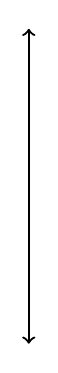
\begin{tikzpicture}
      \draw[<->, thick] (0,1)--(0,5);
      \vspace{1cm}
    \end{tikzpicture}
  }



  % ---------------------- CONNEXIONNISTE ------------------------
  \multirow{3}{*}{\vspace{-6.5cm}\textbf{$\sim$ \textit{Connexionniste}}}
  \vspace{-0.35cm}
                               & \textbf{Maintien cohérence simulation/réel}
  (Sim2Real, Domain Rand.)
                               & $\sim$~--~\cmark                                     & n/a                   & \cmark            & $\sim$             & $\sim$                                     \\

                               & \textbf{Contraintes organisationnelles en MARL}
  (Shielding, Shaping, Constrained-RL)
                               & \xmark~--~$\sim$                                     & $\sim$~--~\cmark      & $\sim$            & \cmark             & $\sim$~--~\cmark                           \\

                               & \textbf{Extraction organisationnelle émergente}
  (ROMA, unsupervised ML...)
                               & \xmark~--~$\sim$                                     & $\sim$                & $\sim$            & \xmark~--~$\sim$   & \cmark                                     \\
  \hline
\end{tabular}
